\documentclass{article}
\usepackage[utf8]{inputenc} %кодировка
\usepackage[T2A]{fontenc}
\usepackage[english,russian]{babel} %русификатор 
\usepackage{mathtools} %библиотека матеши
\usepackage[left=1cm,right=1cm,top=2cm,bottom=2cm,bindingoffset=0cm]{geometry} %изменение отступов на листе
\usepackage{amsmath}
\usepackage{graphicx} %библиотека для графики и картинок
\graphicspath{}
\DeclareGraphicsExtensions{.pdf,.png,.jpg}
\usepackage{subcaption}
\usepackage{pgfplots}
\usepackage{float}
\usepackage{listings}


\lstset{
    numbers=left,            % Нумерация строк слева
    numberstyle=\tiny,       % Размер шрифта для номеров строк
    stepnumber=1,            % Нумеровать каждую строку
    numbersep=5pt,           % Расстояние между номерами и кодом
    backgroundcolor=\color{white},  % Цвет фона
    showspaces=false,        % Не показывать пробелы
    showstringspaces=false,  % Не показывать пробелы в строках
    showtabs=false,          % Не показывать табуляцию
    frame=single,            % Рамка вокруг кода
    tabsize=2,               % Размер табуляции
    breaklines=true,         % Автоматический перенос строк
    breakatwhitespace=true   % Переносить строки только по пробелам
}

\begin{document}
% НАЧАЛО ТИТУЛЬНОГО ЛИСТА
\begin{center}
    \Large
    Федеральное государственное автономное \\
    образовательное учреждение высшего образования \\ 
    «Научно-образовательная корпорация ИТМО»\\
    \vspace{0.5cm}
    \large
    Факультет программной инженерии и компьютерной техники \\
    Направление подготовки 09.03.04 Программная инженерия \\
    \vspace{1cm}
    \Large
    \textbf{Отчёт по лабораторной работе №2} \\
        По дисциплине «Системы ввода-вывода» ( семестр 6)\\
    \large
    \vspace{8cm}

    \begin{minipage}{.33\textwidth}
    \end{minipage}
    \hfill
    \begin{minipage}{.4\textwidth}
    
        \textbf{Студент}: \vspace{.1cm} \\
        \ Дениченко Александр P3312\\
        \ Разинкин Александр P3307\\
        \textbf{Практик}:  \\
        \ Табунщик Сергей Михайлович
    \end{minipage}
    \vfill
Санкт-Петербург\\ 2025 г.
\end{center}
\pagestyle{empty}
% КОНЕЦ ТИТУЛЬНОГО ЛИСТА 
\newpage
\pagestyle{plain}

\section*{Цель}
Познакомится с основами разработки драйверов устройств с
использованием операционной системы на примере создания
драйверов символьных устройств под операционную систему Linux.
\section{Задачи}
Написать драйвер символьного устройства, удовлетворяющий
требованиям:

• должен создавать символьное устройство /dev/varN, где N – это
номер варианта

• должен обрабатывать операции записи и чтения в соответствии с
вариантом задания

\section{Вариант}

При записи текста в файл символьного устройства должно
запоминаться количество пробелов во введенном тексте.
Последовательность полученных результатов с момента
загрузки модуля ядра должна выводиться при чтении файла.

\section{Выполнение}

Функция my\_read является обработчиком системного вызова read() для данного символьного устройства:

\begin{lstlisting}[caption={my\_read}, label={lst:example}]
static ssize_t my_read(struct file *f, char __user *buf, size_t len, loff_t *off)
{
    printk(KERN_INFO "Driver: read()\n");

    result *curr_res;
    int ptr = 0;

    curr_res = first_result;
    while (curr_res) {
        ptr += sprintf(lbuf + ptr, "%ld ", curr_res->spaces);
        curr_res = curr_res->next;
    }

    lbuf[ptr++] = '\n';
    lbuf[ptr++] = '\0';

    size_t count = strlen(lbuf);

    if (*off > 0 || len < count) {
        return 0;
    }

    if (copy_to_user(buf, lbuf, count) != 0) {
        return -EFAULT;
    }

    *off = count;

    return count;
}
\end{lstlisting}
Проходит по связному списку результатов, формирует строку, содержащую все значения, разделенные пробелами.
Копирует данные в пользовательское пространство.
Обновляет смещение в файле и возвращает количество скопированных байт.
\\ \\ \\ \\
Функция my\_write является обработчиком системного вызова write() для данного символьного устройства:
\begin{lstlisting}[caption={my\_write}, label={lst:example}]
static ssize_t my_write(struct file *f, const char __user *buf,  size_t len, loff_t *off)
{
  printk(KERN_INFO "Driver: write()\n");

  if (len > BUF_SIZE) {
    return 0;
  }

  if (copy_from_user(lbuf, buf, len) != 0) {
    return -EFAULT;
  }

  result *res = (result *) kmalloc(sizeof(result), GFP_KERNEL);
  if (!res) {
    printk(KERN_ERR "Can not allocate memory for driver data.\n");
    return 0;
  }

  size_t size = strlen(lbuf);
  size_t spaces = 0;
  size_t i = 0;
  while (i != size) {
    if (lbuf[i] == ' ') {
      spaces++;
    }
    i++;
  }

  res->spaces = spaces;

  if (!last_result) {
    first_result = res;
    last_result = res;
  } else  {
    last_result->next = res;
    last_result = res;
  }
  res->next = NULL;

  return len;
}
\end{lstlisting}
Проверяет, не превышает ли размер данных размер буфера.
Копирует данные из пользовательского пространства в буфер ядра. 
Подсчитывает количество пробелов в полученной строке.
Сохраняет результат в конец связного списка результатов и возвращает кол-во записанных байт.

\section{Полный код}

\begin{lstlisting}[caption={ch\_drv.c}, label={lst:example}]
#include <linux/module.h>
#include <linux/version.h>
#include <linux/kernel.h>
#include <linux/types.h>
#include <linux/kdev_t.h>
#include <linux/fs.h>
#include <linux/device.h>
#include <linux/cdev.h>
#include <linux/slab.h>

#define BUF_SIZE 256

static dev_t first;
static struct cdev c_dev; 
static struct class *cl;

static char lbuf[BUF_SIZE];

typedef struct result {
  size_t spaces;
  struct result *next;
} result;

static result *first_result, *last_result;

static int my_open(struct inode *i, struct file *f)
{
  printk(KERN_INFO "Driver: open()\n");
  return 0;
}

static int my_close(struct inode *i, struct file *f)
{
  printk(KERN_INFO "Driver: close()\n");
  return 0;
}

static ssize_t my_read(struct file *f, char __user *buf, size_t len, loff_t *off)
{
  printk(KERN_INFO "Driver: read()\n");

  result *curr_res;
  int ptr = 0;

  curr_res = first_result;
  while (curr_res) {
    ptr += sprintf(lbuf + ptr, "%ld ", curr_res->spaces);
    curr_res = curr_res->next;
  }

  lbuf[ptr++] = '\n';
  lbuf[ptr++] = '\0';

  size_t count = strlen(lbuf);

  if (*off > 0 || len < count) {
    return 0;
  }

  if (copy_to_user(buf, lbuf, count) != 0) {
    return -EFAULT;
  }

  *off = count;

  return count;
}

static ssize_t my_write(struct file *f, const char __user *buf,  size_t len, loff_t *off)
{
  printk(KERN_INFO "Driver: write()\n");

  if (len > BUF_SIZE) {
    return 0;
  }

  if (copy_from_user(lbuf, buf, len) != 0) {
    return -EFAULT;
  }

  result *res = (result *) kmalloc(sizeof(result), GFP_KERNEL);
  if (!res) {
    printk(KERN_ERR "Can not allocate memory for driver data.\n");
    return 0;
  }

  size_t size = strlen(lbuf);
  size_t spaces = 0;
  size_t i = 0;
  while (i != size) {
    if (lbuf[i] == ' ') {
      spaces++;
    }
    i++;
  }

  res->spaces = spaces;

  if (!last_result) {
    first_result = res;
    last_result = res;
  } else  {
    last_result->next = res;
    last_result = res;
  }
  res->next = NULL;

  return len;
}

static struct file_operations mychdev_fops =
{
  .owner = THIS_MODULE,
  .open = my_open,
  .release = my_close,
  .read = my_read,
  .write = my_write
};
 
static int __init ch_drv_init(void)
{
    printk(KERN_INFO "Hello!\n");
    if (alloc_chrdev_region(&first, 0, 1, "ch_dev") < 0){
            return -1;
    }
    if ((cl = class_create(THIS_MODULE, "chardrv")) == NULL){
            unregister_chrdev_region(first, 1);
            return -1;
    }
    if (device_create(cl, NULL, first, NULL, "mychdev") == NULL){
            class_destroy(cl);
            unregister_chrdev_region(first, 1);
            return -1;
    }
    cdev_init(&c_dev, &mychdev_fops);
    if (cdev_add(&c_dev, first, 1) == -1){
            device_destroy(cl, first);
            class_destroy(cl);
            unregister_chrdev_region(first, 1);
            return -1;
    }
    return 0;
}
 
static void __exit ch_drv_exit(void)
{
    cdev_del(&c_dev);
    device_destroy(cl, first);
    class_destroy(cl);
    unregister_chrdev_region(first, 1);
    printk(KERN_INFO "Bye!!!\n");
}
 
module_init(ch_drv_init);
module_exit(ch_drv_exit);
 
MODULE_LICENSE("GPL");
MODULE_AUTHOR("Author");
MODULE_DESCRIPTION("The first kernel module");
\end{lstlisting}


\end{document}
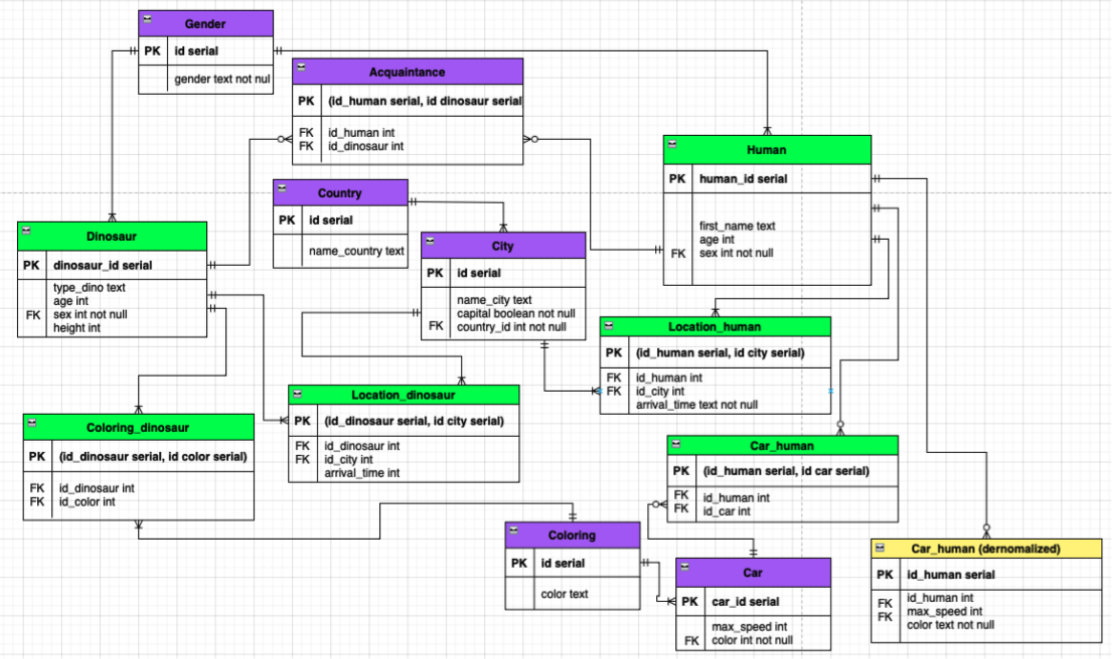
\includegraphics[width=.9\textwidth]{123}
\begin{lstlisting}[caption={kernel.ld}, label={lst:example}]
    
\end{lstlisting}
